\chapter*{Lab 4 - Ray Tracing}

\section{Parte 1 - openGL}
In questa esercitazione si richiedeva di implementare la gestione dei seguenti elementi:
\textbf{\begin{itemize}
  \item Shadow Rays
  \item Reflection Rays
  \item Soft Shadows
\end{itemize}}

L'algoritmo di Ray Tracing viene richiamato alla pressione del tasto R della tastiera e viene richiamato per ogni pixel della viewport. La funzione TraceRay crea un oggetto Hit che serve per determinare il punto di incidenza con la scena. Questo oggetto deve essere fornito alla funzione CastRay che crea effettivamente il raggio e provoca l'intersezione di questo raggio con un oggetto della scena. La classe RayTree viene richiamata in questo punto e  permette di disegnare i diversi raggi primari, riflessi e d'ombra alla pressione del tasto T. 

L'algoritmo vero e proprio comincia con la creazione del colore di risposta riempito inizialmente con il colore del background. In caso in cui non vi sia alcuna intersezione, l'algoritmo ritorna questo colore, altrimenti procede con l'aggiunta di tutti i contributi luminosi. Si ricavano tutti i valori utili al materiale, punto di intersezione e normale alla superficie nel punto di intersezione. Se il materiale intersecato è emittente, allora si ritorna direttamente il colore della luce senza effettuare altri calcoli.
Successivamente si procede con la logica delle ombre.

\subsection{Shadow Logic}
Quando si esegue l'applicativo è possibile definire il numero di campioni d'ombra che si devono prendere, con il parametro \texttt{num\_shadow\_samples}. Quindi l'algoritmo per ogni luce della scena ripete la logica un numero di volte pari a questo parametro e poi fa la media di tutti i contributi che ottiene. La logica distingue i casi in cui il numero di campioni da ottenere sia pari a 0 o maggiore di 0. Se è 0 allora non vi devono essere ombre, quindi si lascia ciò che era già nel template: si fa direttamente il calcolo di Phong con la funzione \texttt{Shade} per ottenere il colore dell'oggetto intersecato dipendentemente dal colore e dall'intensità della luce.

Se invece vi è almeno un campione d'ombra, è necessario creare uno shadow ray 
	che parta dal punto di incidenza sulla scena e che abbia come direzione la luce attualmente considerata. A questo punto, si calcola il punto di incidenza nuovo e si confronta la lunghezza del nuovo raggio con la distanza dalla luce. Se sono uguali allora il punto è in luce, altrimenti vi è qualcosa in mezzo e questo punto non ottiene il contributo luminoso della luce considerata. Se la distanza è praticamente la stessa, allora si applica il contributo richiamando \texttt{Shade}.\\

Un esempio del risultato dopo l'applicazione di un campione d'ombra:
\begin{figure}[htb]
    \centering
    \vspace{-0.7cm}
    \subfloat[]{{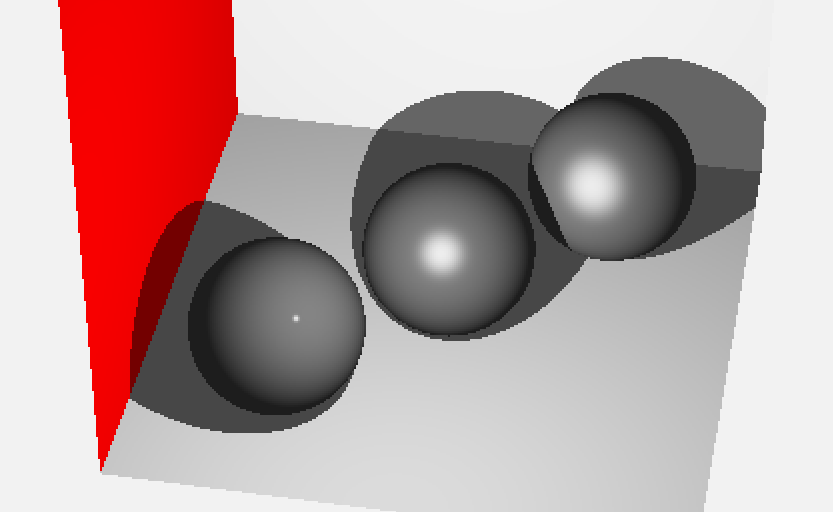
\includegraphics[height=4cm]{shadow1} }}%
    \subfloat[]{{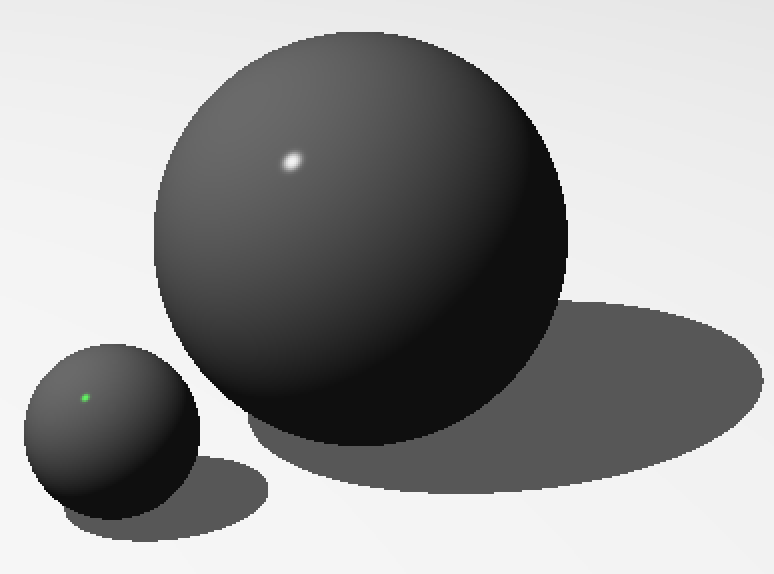
\includegraphics[height=4cm]{shadow2} }}%
    \vspace{-0.3cm}
\end{figure}

\subsection{Reflection Logic}
\begin{wrapfigure}{l}{0.5\textwidth} %this figure will be at the right
    \centering
    \vspace{-0.5cm}
    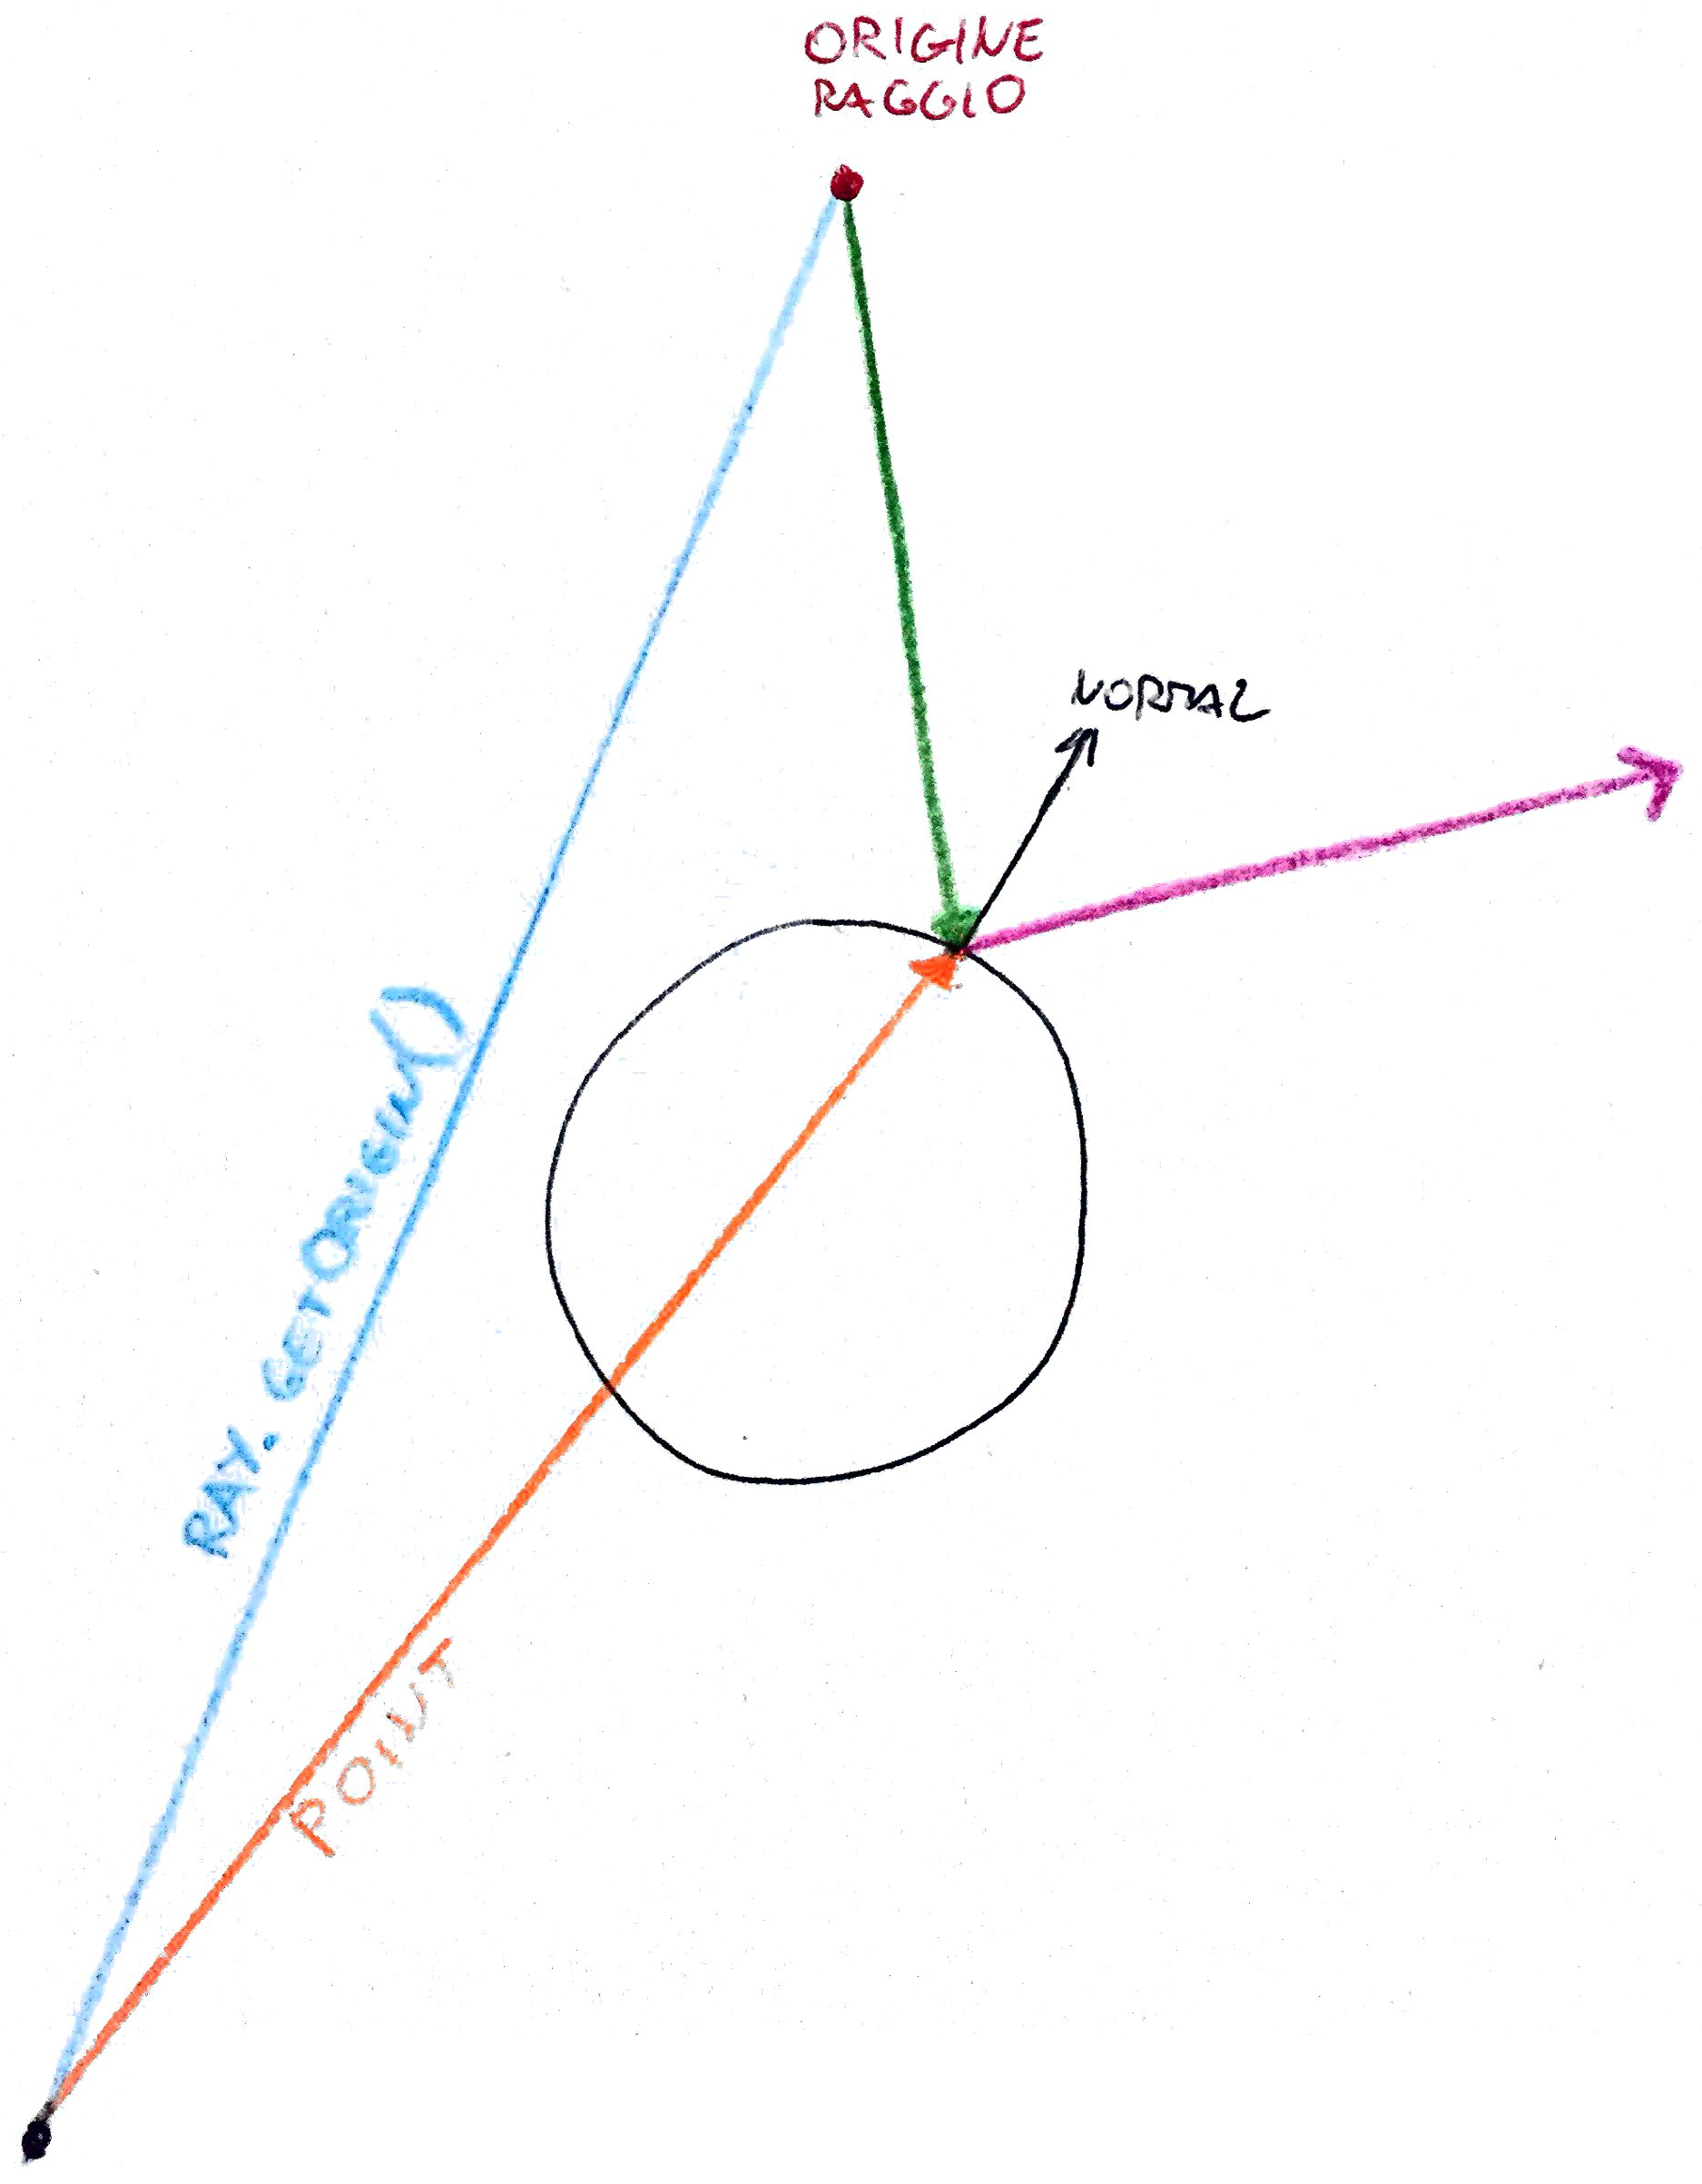
\includegraphics[height=8cm]{point}
    
    \caption{\label{fig:point}}
\end{wrapfigure} 
    La logica dei riflessi è molto più semplice: prima di tutto si controlla se vi è una componente riflettente nel materiale dell'oggetto intersecato.\\ 
    Se l'oggetto non è riflettente l'algoritmo termina, altrimenti si calcola il raggio riflesso e ricorsivamente si richiama \texttt{TraceRay} con il nuovo raggio finché vi sono rimbalzi (\texttt{num\_bounces}).\\
    Nell'immagine \ref{fig:point} è illustrata la situazione di un raggio incidente (verde) e il suo riflesso (viola). Il raggio incidente è ottenibile con la differenza tra il vettore \textit{point} e il vettore che rappresenta l'origine del raggio.\\

Il raggio riflesso è ottenibile con la formula
\begin{center}
	$R=2<n, l> n - l$
\end{center}
ovvero due volte il prodotto scalare tra normale e raggio incidente, moltiplicato per la normale; il vettore risultante deve essere sottratto al raggio incidente.

\begin{figure}[hbt]
    \centering
    \vspace{-0.2cm}
    \subfloat[Due sfere riflettive]{{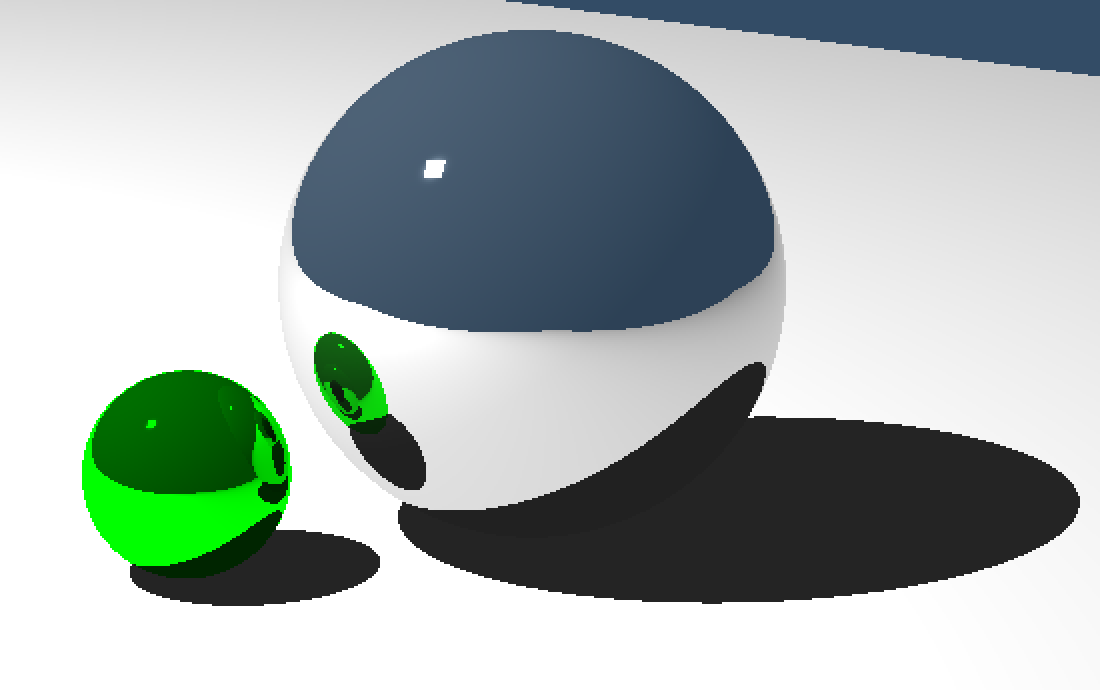
\includegraphics[height=4cm]{ray1} }}%
    \subfloat[Background più chiaro]{{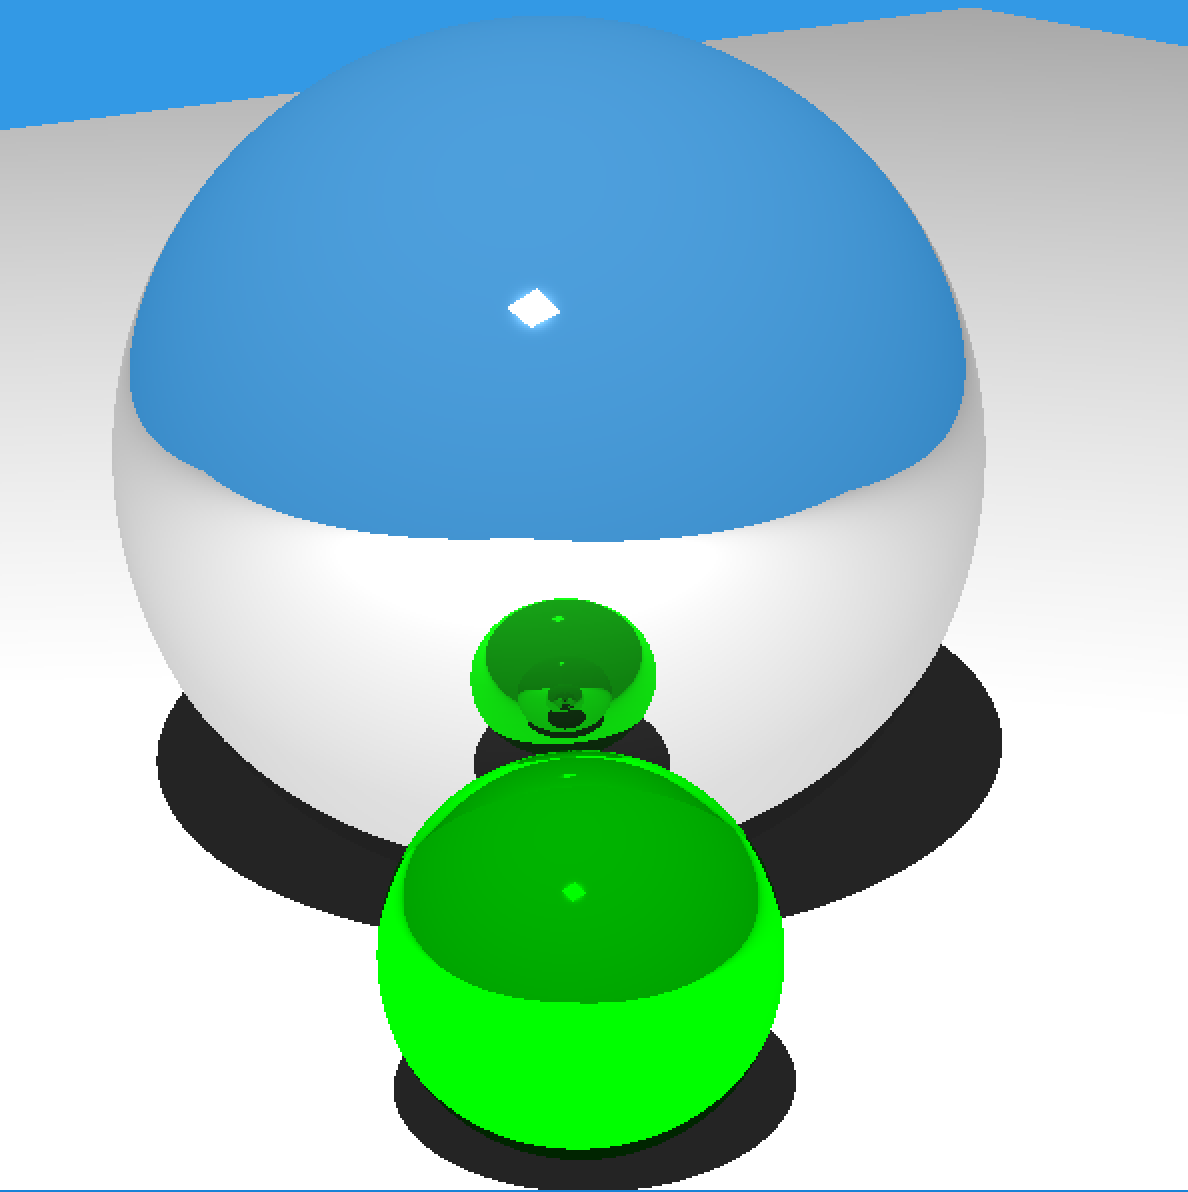
\includegraphics[height=4cm]{ray2} }}%
    \subfloat[RayTree di debug]{{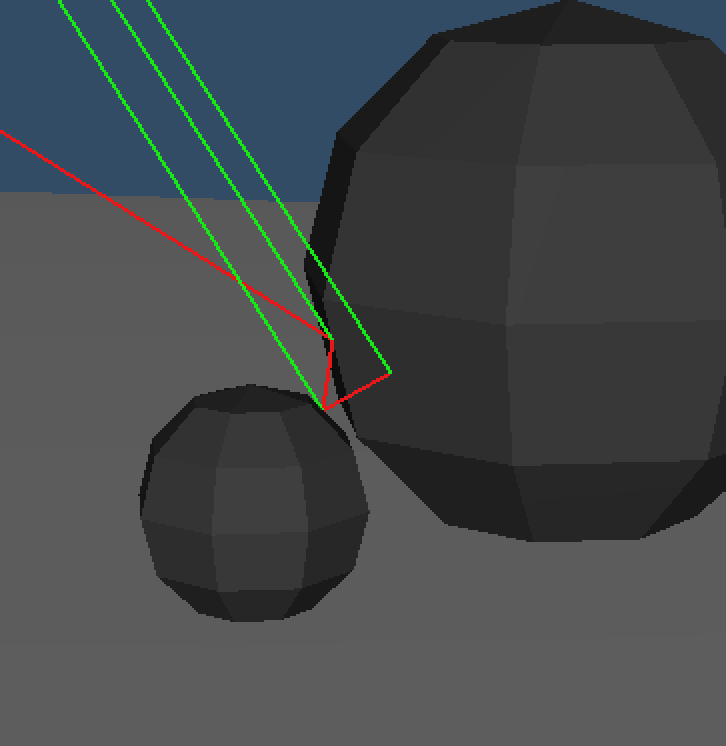
\includegraphics[height=4cm]{ray3} }}%
	\vspace{-0.5cm}
\end{figure}\footnote{(Nota: fin da subito è stato modificato il file \texttt{reflective\_\-spheres.obj} sostituendo il colore rosso riflettente con il verde)}


\newpage
\subsection{Soft Shadows}
Le soft-shadows sono state ottenute modificando la logica delle ombre e tracciando tanti raggi che intersecano randomicamente l'area della luce considerata quanto indicato con il parametro \texttt{num\_\-shadow\_\-samples}. Ogni contributo viene sommato e al termine del ciclo che interseca tutti gli shadow ray viene fatta la media di questi contributi.

\begin{figure}[hbt]
	\vspace{-0.3cm}
    \centering
    \subfloat[4 campionature]{{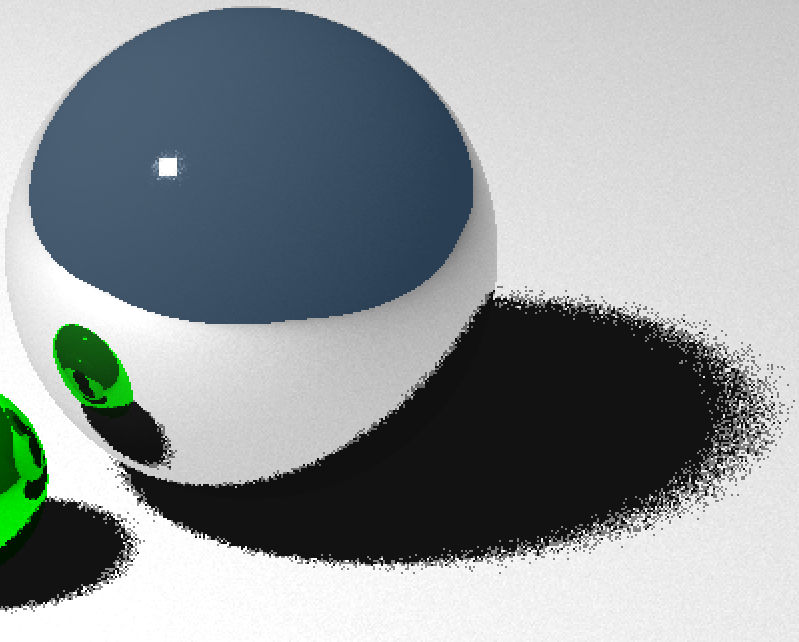
\includegraphics[height=4cm]{soft1} }}%
    \subfloat[16 campionature]{{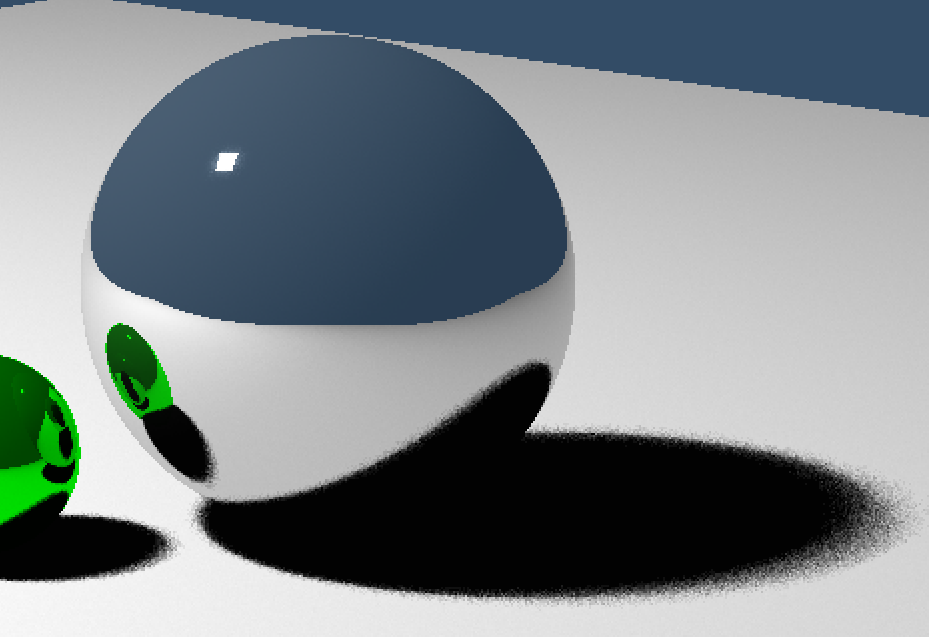
\includegraphics[height=4cm]{soft2} }}%
    \subfloat[RayTree di debug]{{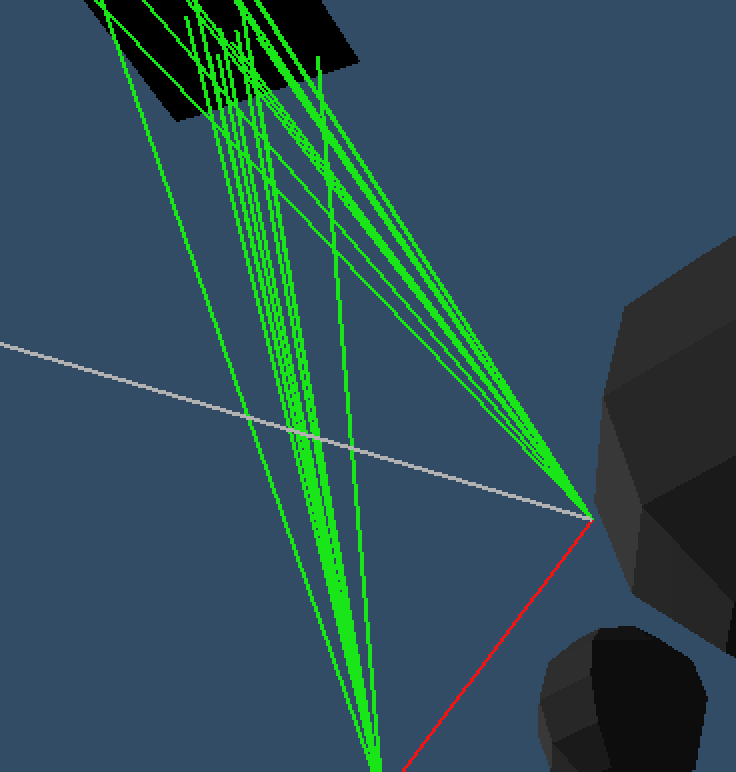
\includegraphics[height=4cm]{soft3} }}%
	\vspace{-0.7cm}
\end{figure}

\subsubsection{Antialiasing}
Per avere un migliore riscontro visivo nella rappresentazione delle soft-shadow, si è scelto di studiare un metodo per rappresentare un effetto più sfumato e quindi di applicare un filtro di antialiasing. Il metodo più semplice è il seguente: invece di sparare un raggio al centro del pixel attuale, si sparano più raggi in posizioni randomiche e si fa la media dei contributi ottenuti. 

Nella classe \texttt{glCanvas} vi è la funzione \texttt{TraceRay} che richiama l'omonima funzione della classe \texttt{RayTracer}. In questa funzione è stata aggiunta una logica che cicla tante volte quanto specificato nel parametro \texttt{num\_\-antialias\_\-samples} (che è stato aggiunto ad \texttt{argParser.h}). Ad ogni ciclo si randomizza la posizione del raggio e si da in pasto alla funzione \texttt{TraceRay}. Questo algoritmo di antialiasing ha un grande costo computazionale poiché aumenta esponenzialmente il numero di raggi e quindi il tempo di rendering.

\begin{figure}[hbt]
    \centering
    \vspace{-0.2cm}
    \subfloat[Prima]{{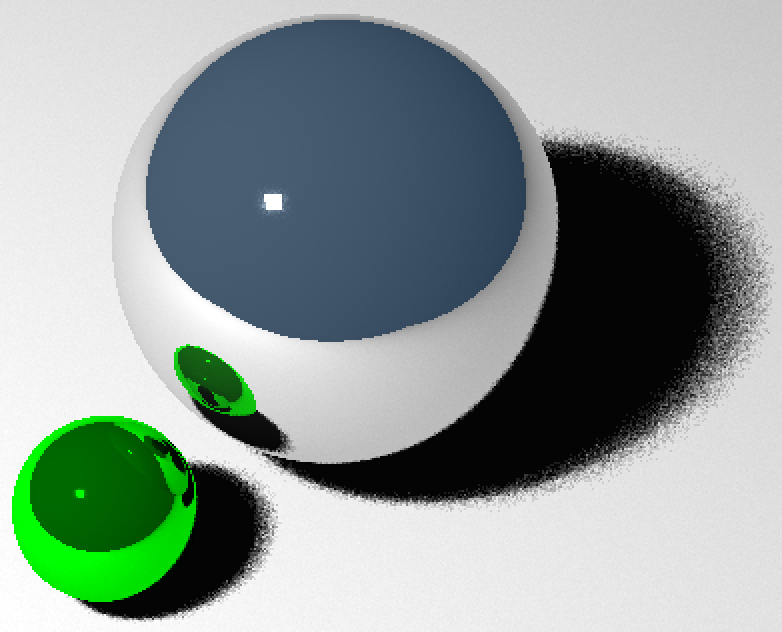
\includegraphics[height=4cm]{anti1} }}%
    \subfloat[Dopo 30 campioni di antialiasing]{{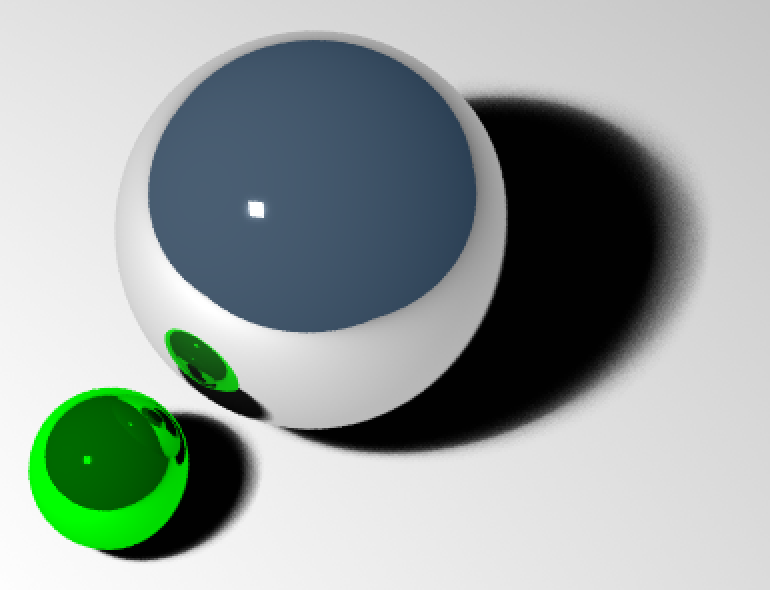
\includegraphics[height=4cm]{anti2} }}%
    \subfloat[RayTree di debug]{{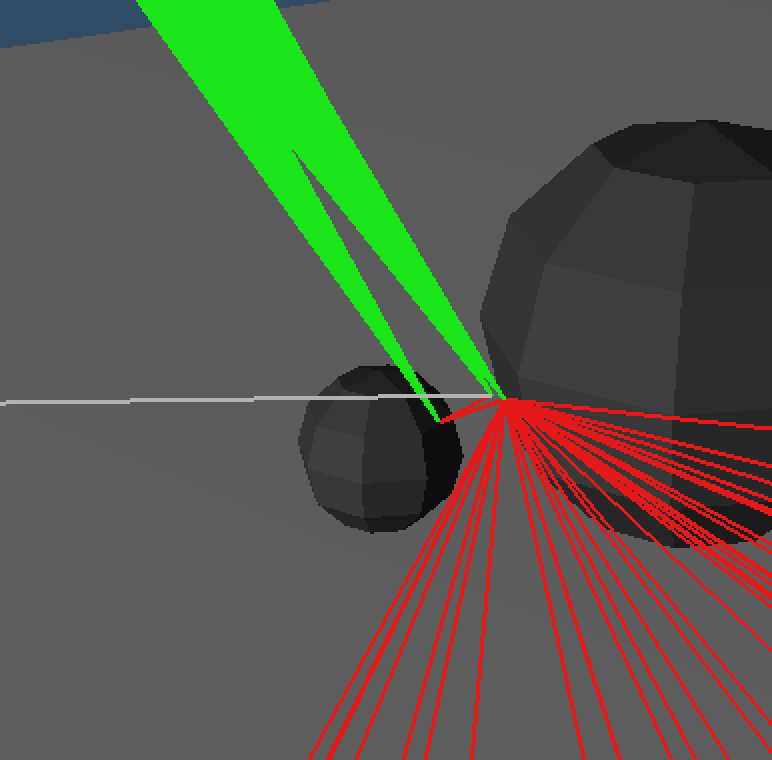
\includegraphics[height=4cm]{anti3} }}%
	\vspace{-0.7cm}
\end{figure}

\subsection{Sperimentazioni}
\begin{figure}[hbt]
    \centering
    \vspace{-0.5cm}
    \subfloat[Due palline verdi]{{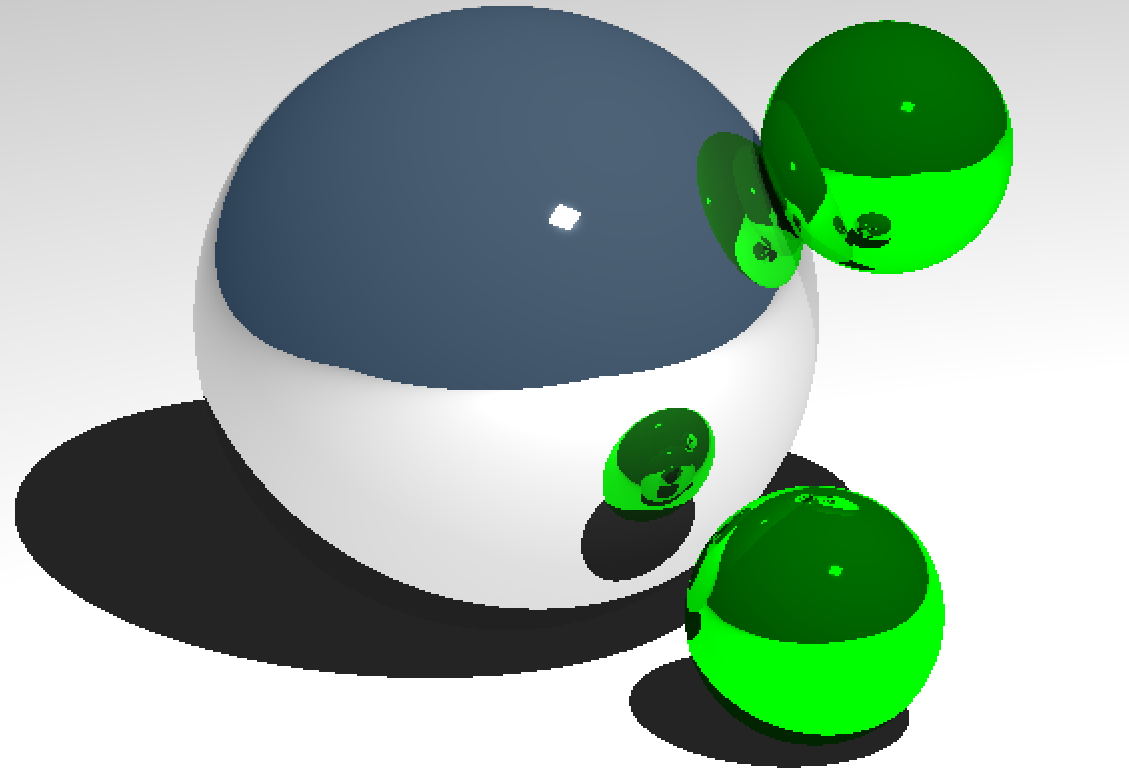
\includegraphics[height=3.8cm]{rand1} }}%
    \subfloat[Due luci]{{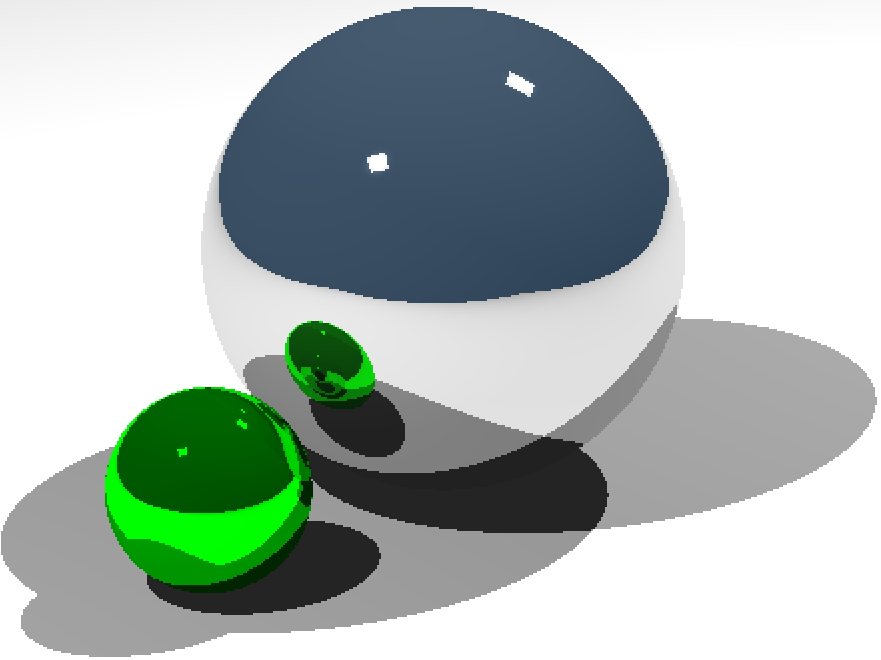
\includegraphics[height=3.8cm]{rand2} }}%
    \subfloat[Tre luci]{{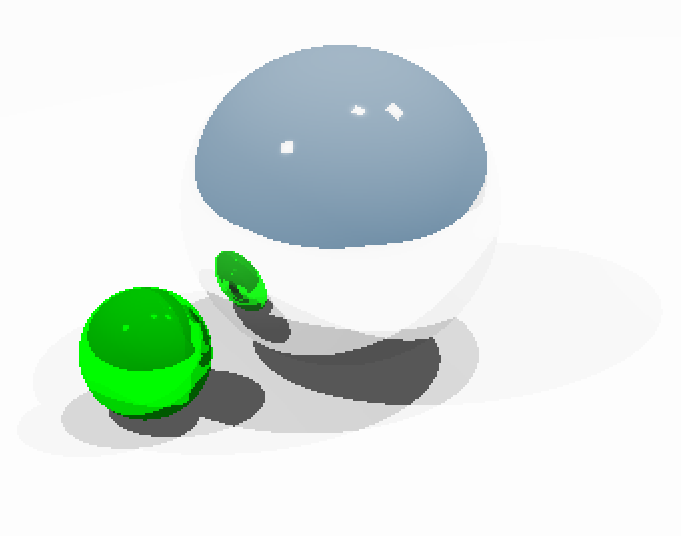
\includegraphics[height=3.8 cm]{rand3} }}%
	\vspace{-0.5cm}
\end{figure}



\newpage
%=============================================================
\section{Parte 2 - Blender}
Per questa parte è stata modificata la scena contenente la batteria cambiando materiali e aggiungendo oggetti riflettenti e trasparenti.

Inizialmente è stato modificato il materiale dei fusti della batteria, selezionando solo la parte delle pelli e rendendola in gran percentuale trasparente attivando la modalità \texttt{Transparency} con un alpha pari a 0.2. In questo modo tutti i fusti hanno almeno due materiali: il bianco dei fusti, il nero dei ring (anelle di ferro che tirano le pelli) e il trasparente delle pelli.

Successivamente sono state aggiunte alla scena 3 NURBS patches a cui è stato applicato il materiale \textit{Specchio} che riflette con un fattore di riflessione dell'80\%. 
\begin{figure}[hbt]
    \centering
    \vspace{-0.5cm}
    \subfloat[Materiale riflettente]{{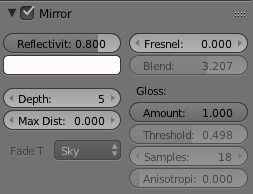
\includegraphics[height=3.8cm]{reflect} }}%
    \subfloat[Materiale trasparente]{{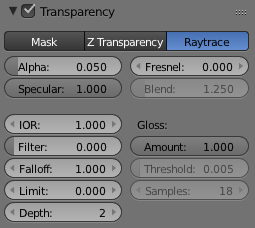
\includegraphics[height=3.8cm]{transparent} }}%
	\vspace{-0.5cm}
\end{figure}


Tutta la scena è stata rinchiusa in un grande cilindro con materiale rosso che crea una sorta di stanza ed è stata illuminata con una luce centrale bianca.

 \begin{figure}[htb]
    \centering
    %\vspace{-0.7cm}
    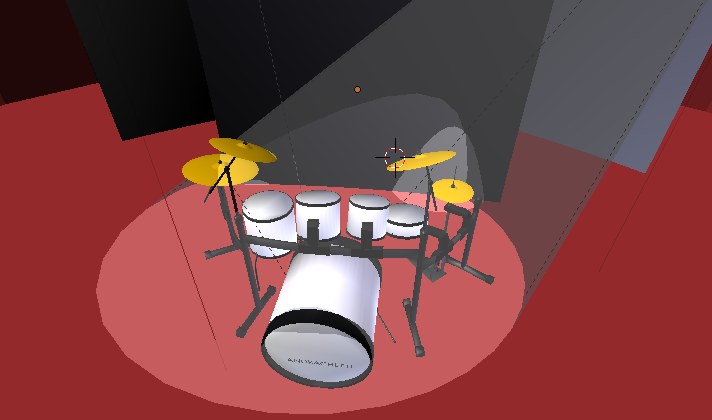
\includegraphics[width=\textwidth]{scene1}
    \caption{\label{fig:scene1}}
    %\vspace{-0.3cm}
\end{figure}

Successivamente, la scena è stata arricchita con due oggetti posizionati dietro lo specchio centrale. A sinistra è stata posizionata una sfera con materiale riflettente e una luce blu che la illumina; mentre a destra è stato posizionato un toro con material trasparente con una luce verde che lo illumina dall'alto.
\newpage

La scena prima del render non presenta le trasparenze, né i riflessi:
 \begin{figure}[htb]
    \centering
    %\vspace{-0.3cm}
    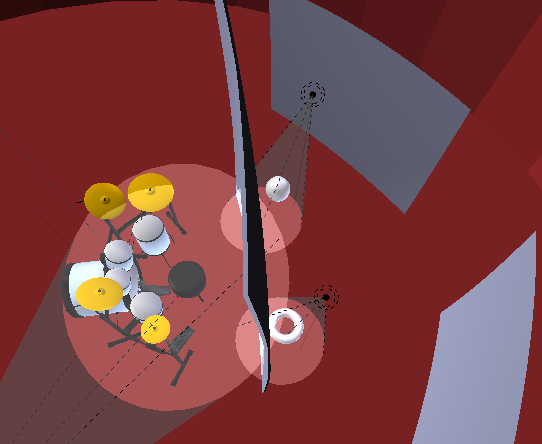
\includegraphics[width=0.6\textwidth]{scene2}
    \caption{\label{fig:scene2}}
    \vspace{-0.3cm}
\end{figure}

Il risultato del render invece porta con se tutti gli effetti speciali dovuti ai materiali e alle luci:
 \begin{figure}[htb]
    \centering
    %\vspace{-0.7cm}
    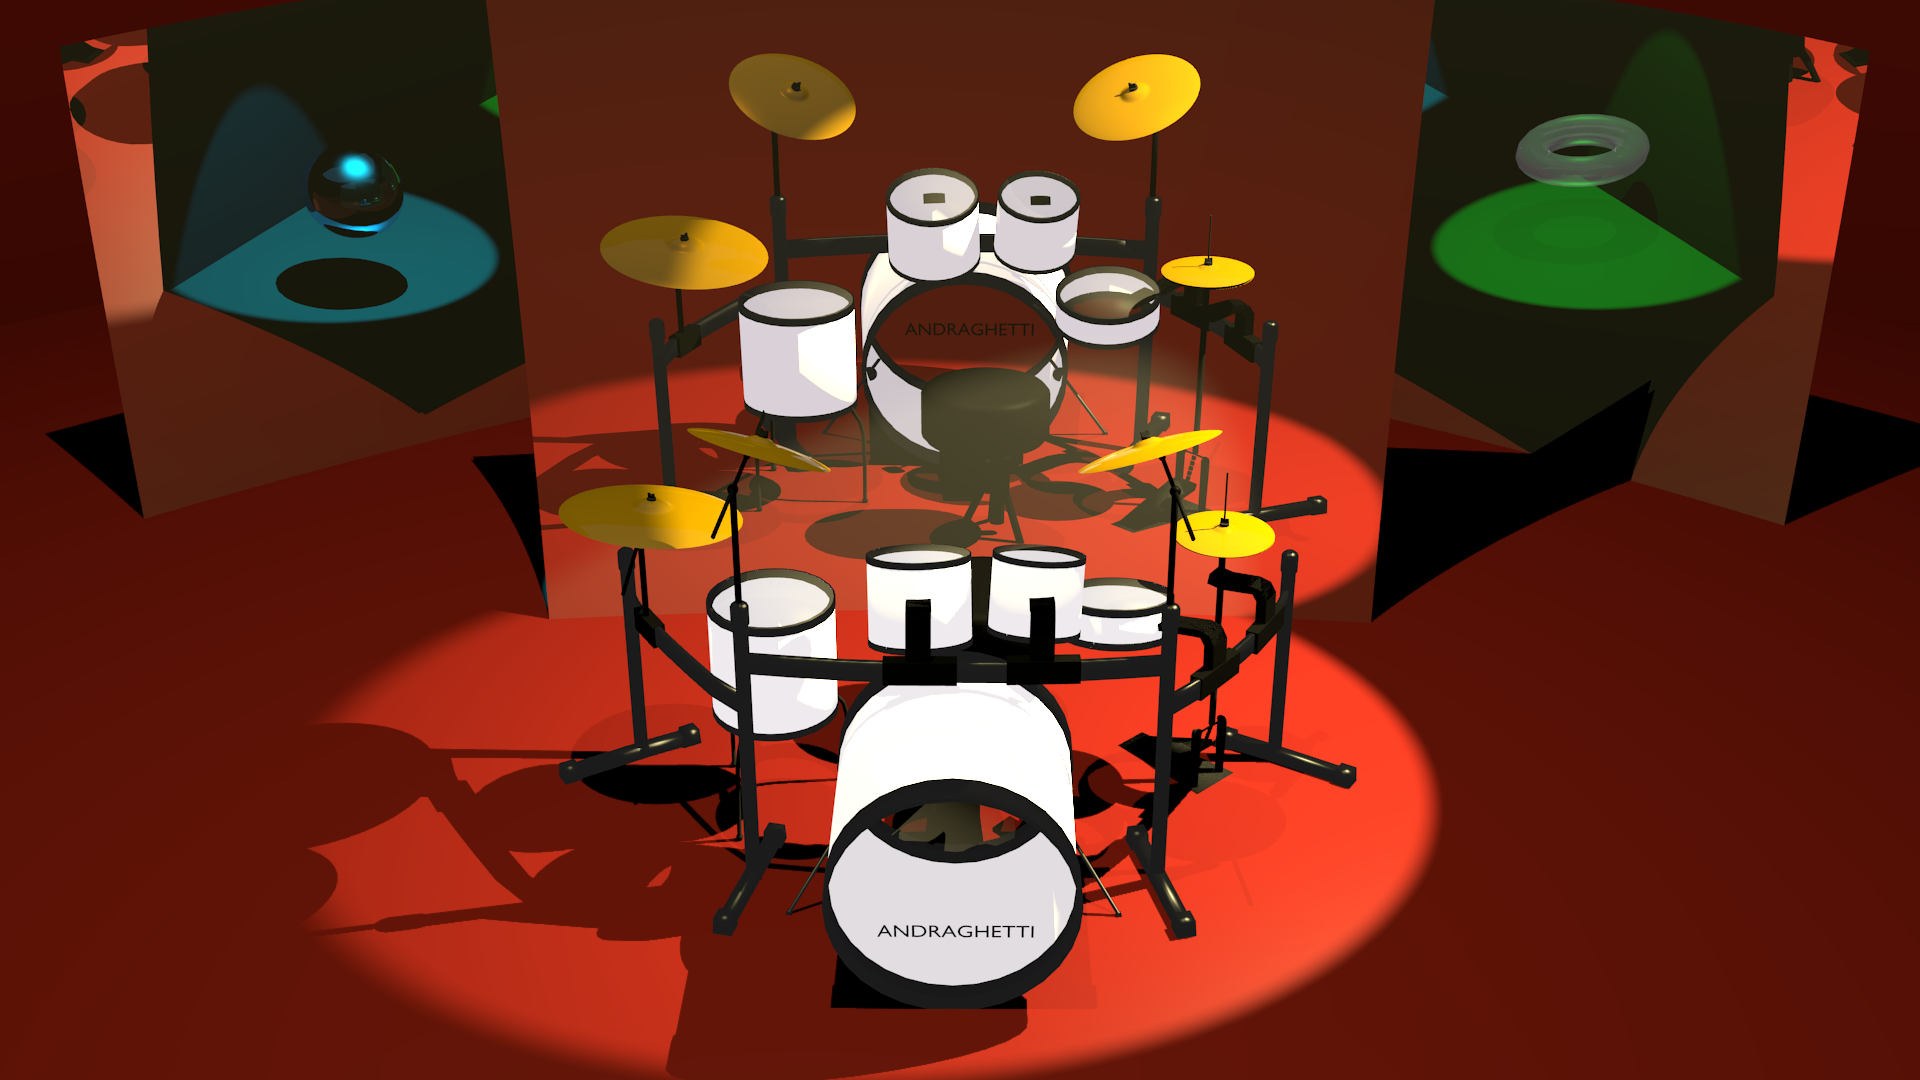
\includegraphics[width=\textwidth]{render}
    \caption{\label{fig:render}}
    \vspace{-0.7cm}
\end{figure}


























%

